% !TEX root = ../../../main.tex

\toggletrue{image}
\toggletrue{imagehover}
\chapterimage{data}
\chapterimagetitle{\uppercase{Data}}
\chapterimageurl{https://xkcd.com/1492/}
\chapterimagehover{If you want to have more fun at the expense of language pedants, try developing an hypercorrection habit.}

%https://cgvr.informatik.uni-bremen.de/teaching/info1_0506/folien/02_repraesentation_daten_2up_1.pdf
%https://files.ifi.uzh.ch/ee/fileadmin/user_upload/teaching/hs12/02_FGI_Information_Text.pdf
%https://pbs.twimg.com/media/Dcb3tbSXUAAWr4H?format=jpg&name=large
%https://www.meteoschweiz.admin.ch/home/messwerte.html?param=messwerte-lufttemperatur-10min&station=LAE&chart=hour
%https://upload.wikimedia.org/wikipedia/commons/thumb/a/ab/Tacho_100tkm.JPG/768px-Tacho_100tkm.JPG

\chapter{Daten}
\label{chapter-daten}

In diesem Kapitel klären wir, was man unter dem Begriff Daten versteht. Wir werden dann den Unterschied zwischen analogen und digitalen Daten betrachten. Der Fokus wird jedoch immer auf den digitalen Daten liegen. Dies aus einem einfachen Grund: der Computer verarbeitet digitale Daten. Die Lernziele lauten:

\newcommand{\datenLernziele}{
\protect\begin{todolist}
\item Sie definieren den Begriff Daten.
\item Sie erklären den Zusammenhang zwischen Information und Daten.
\item Sie unterscheiden digitale und analoge Daten und geben Beispiele.
\end{todolist}
}

\lernziel{\autoref{chapter-daten}, \nameref{chapter-daten}}{\protect\datenLernziele}

\datenLernziele

%https://www.elektronik-kompendium.de/sites/com/1702271.htm

\section{Was sind Daten?}

Computer verarbeiten \textbf{Daten}. Genauer gesagt: Der Computer arbeitet mit elektronischen Daten\footnote{Die Abkürzung \acs{EDV} ist im deutschsprachigen Raum ein gängiger Begriff.}.

\begin{definition}[Daten]
Daten \say{repräsentieren} Information. Die Daten sind die Träger von Information. Durch eine (maschinelle) Verarbeitung von Daten, können neue Daten erzeugt werden. Man kann bezüglich der Erscheinungsform, der Speicherung und der Aufgabe unterscheiden.
\end{definition}

\begin{example}
Daten können als Schrift, Ton oder Bild in Erscheinung treten. Sie können analog oder digital gespeichert werden. Es gibt zahlreiche Aufgaben. Ein paar Beispiele:

\begin{multicols}{2}
\begin{itemize}
\item Sprachnachrichten
\item Video-Call
\item Adressdaten
\item Steuerdaten
\item Profildaten (z.B. von Instagram)
\item Fotosammlung
\end{itemize}
\end{multicols}

\end{example}

\section{Zusammenhang zwischen Information und Daten}

Daten stellen Information dar. Es ist eine Repräsentation der Information. Oft ist es jedoch so, dass es für eine Information verschiedene Möglichkeiten zur Repräsentation gibt. Somit sind die daraus resultierenden Daten meist \textbf{kein} identisches Abbild der ursprünglichen Information. Häufig wird in diesem Zusammenhang auch der Begriff Wissen hinzugenommen. Die Wissenspyramide aus \autoref{figure-wissenspyramide} zeigt den Zusammenhang der drei Begriffe. Sie bauen aufeinander auf.

\begin{figure}[htb]
\centering
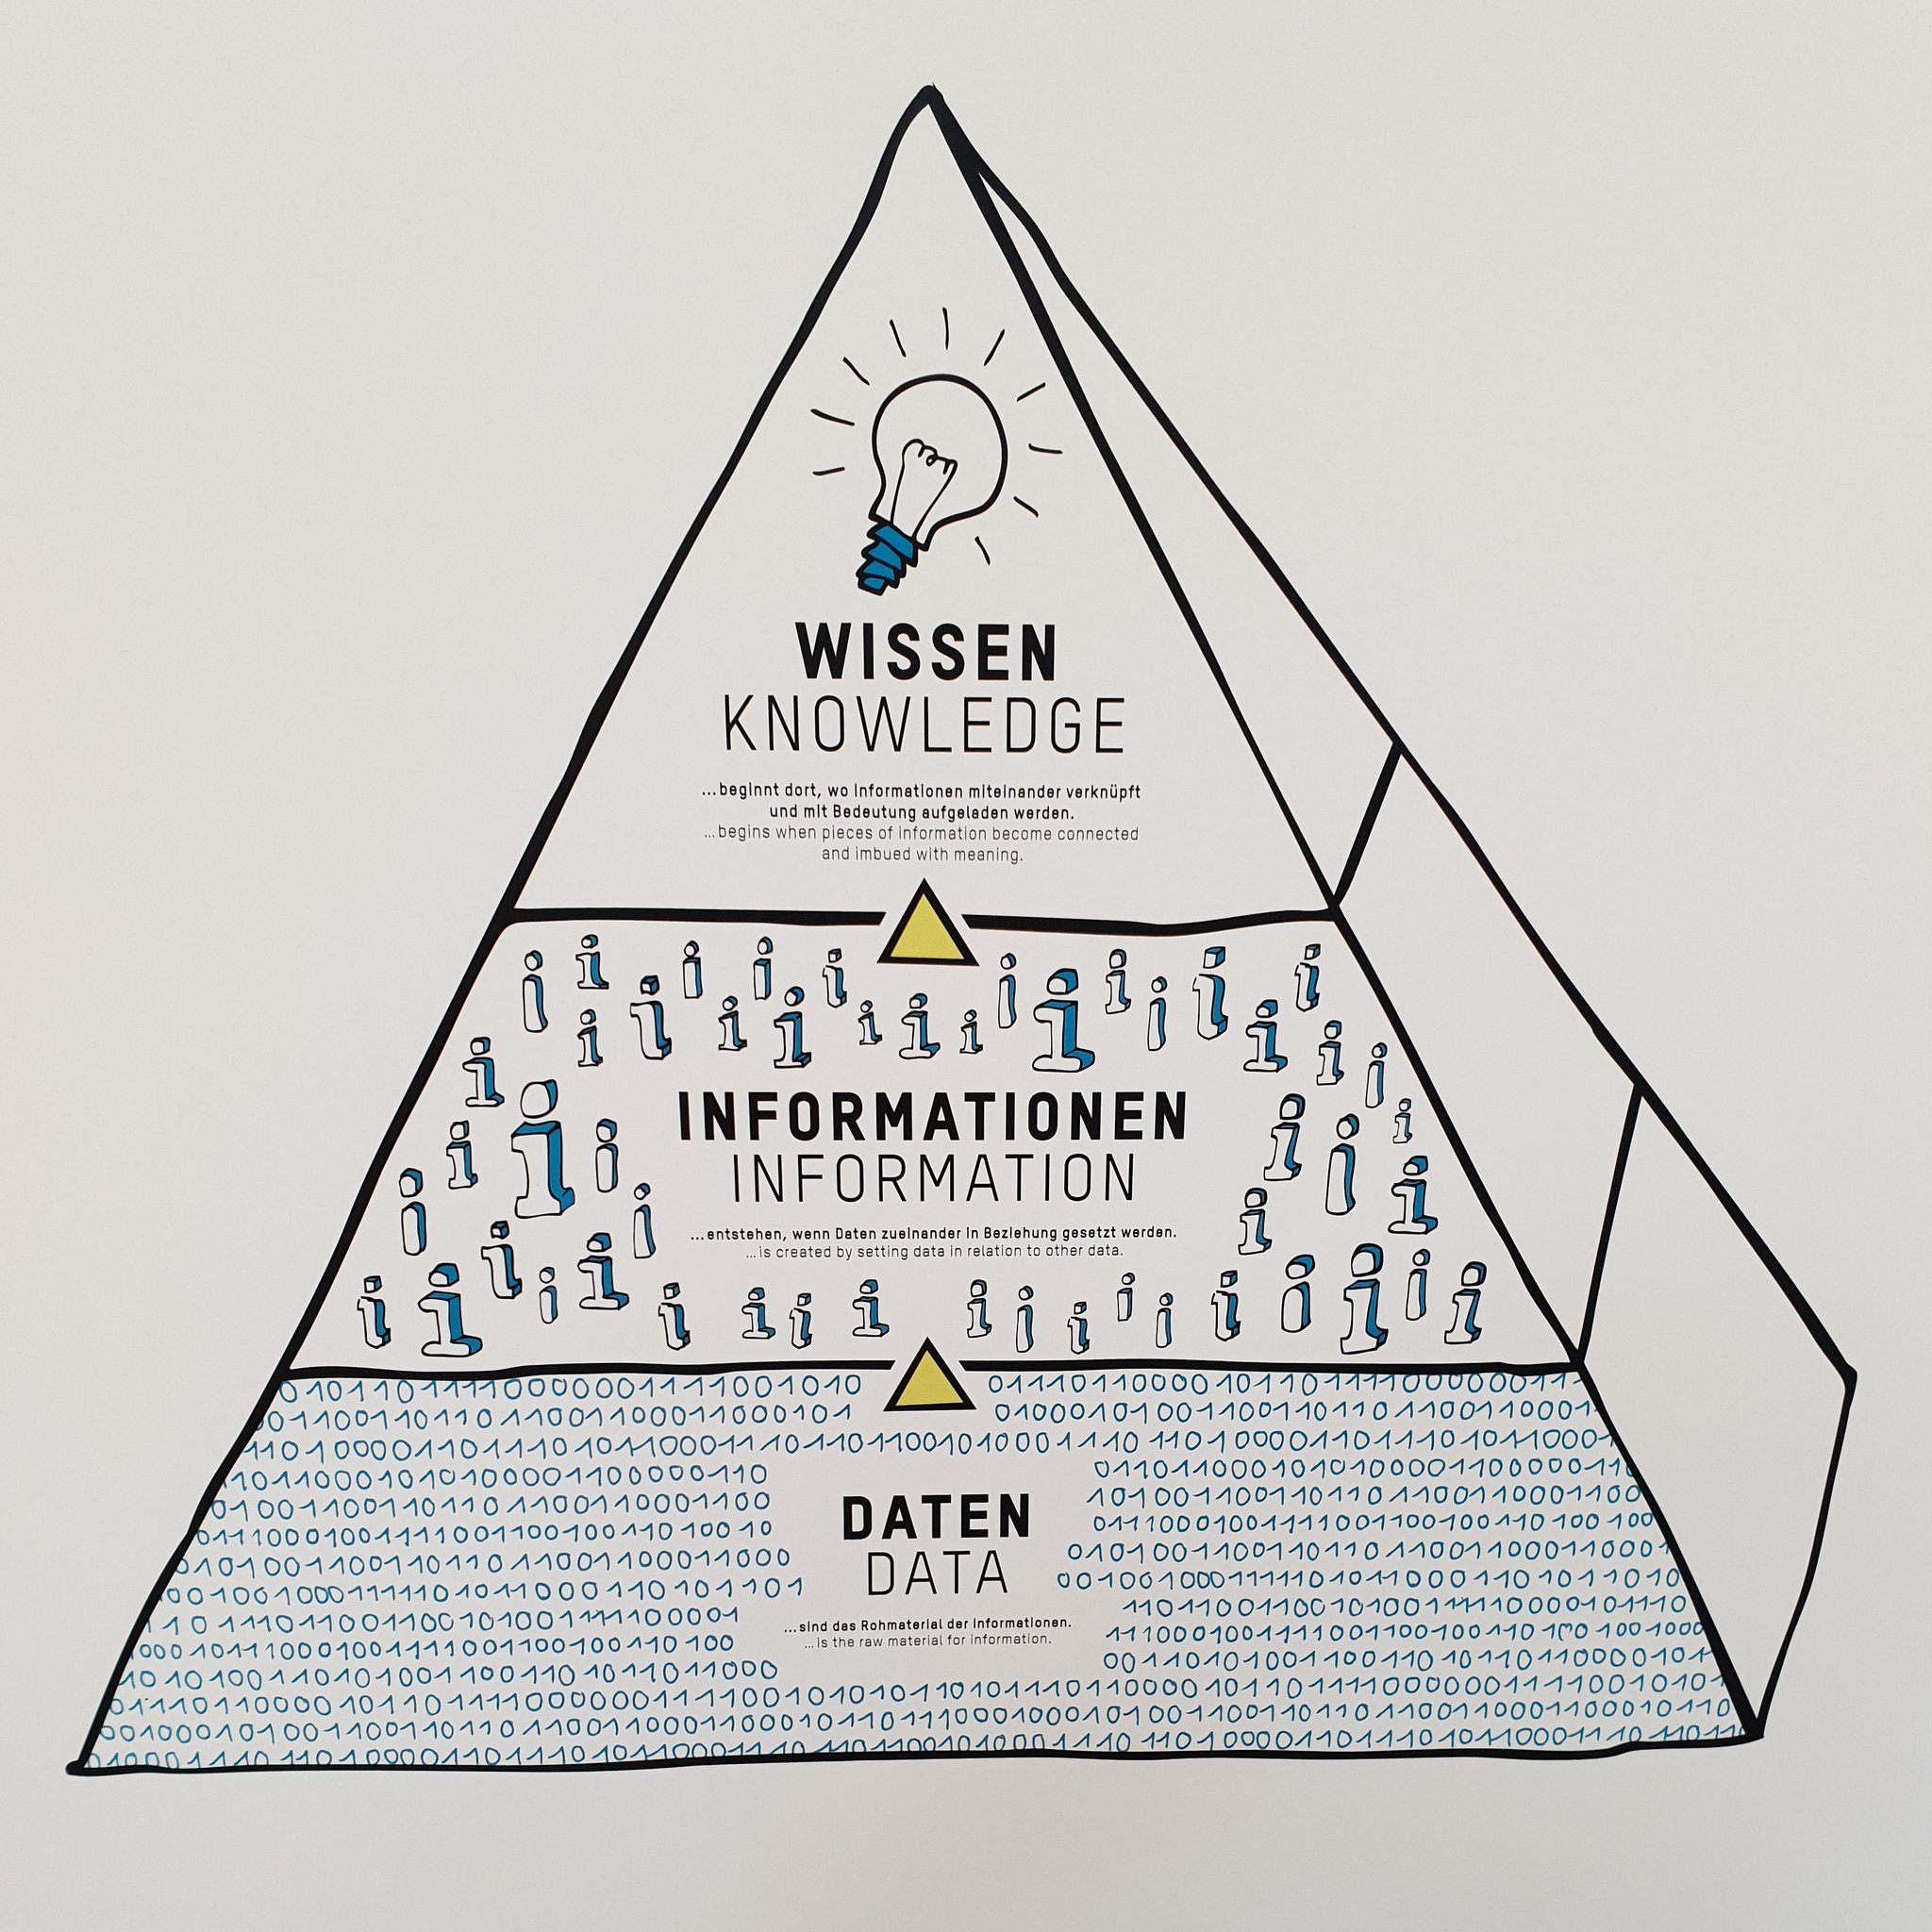
\includegraphics[height=6.75cm]{wissenspyramide.jpeg}
\caption{Zahlen, Buchstaben und Zeichen ergeben nur im Kontext einen Sinn. Informationen werden durch Daten dargestellt. Der Kontext gibt an, was die Daten bedeuten. Wissen wird aus Informationen durch Erfahrung gewonnen.}
\label{figure-wissenspyramide}
\end{figure}

\begin{example}
Die Notenskala der Schulnoten reicht in der Schweiz und in Deutschland von $1$ bis $6$. Die Note $5$ (Daten) benötigen jedoch einen Kontext, damit die korrekte Information daraus gewonnen werden kann. In der Schweiz ist es eine gute Note, in Deutschland wäre es eine ungenügende Note.
\end{example}

\section{Analoge Daten}

Unsere Umwelt liefert analoge Daten. Dies sind physikalische Grössen wie zum Beispiel die Temperatur, das Gewicht oder Schallwellen.

\begin{definition}[Analoge Daten]
Beschreibt eine kontinuierliche Funktion (auch stetige oder stufenlose Funktion genannt) einen Vorgang, dann handelt es sich um analoge Daten. Somit existiert zu jedem Zeitpunkt ein Wert mit einer beliebigen Genauigkeit. Bei einem analogen Vorgang können prinzipiell unendlich viele verschiedene Werte vorkommen.
\end{definition}

Die Definition von analogen Daten ist nicht einfach. Ein paar Beispiele sollen die Idee verdeutlichen.

\begin{example}
Die Lufttemperatur kann durch eine kontinuierliche Funktion beschrieben werden (siehe \autoref{figure-temperaturverlauf}). Die Temperatur macht dabei keine Sprünge, sie ist kontinuierlich. 

\begin{figure}[htb]
\centering
\begin{minipage}{0.6\textwidth}
\centering
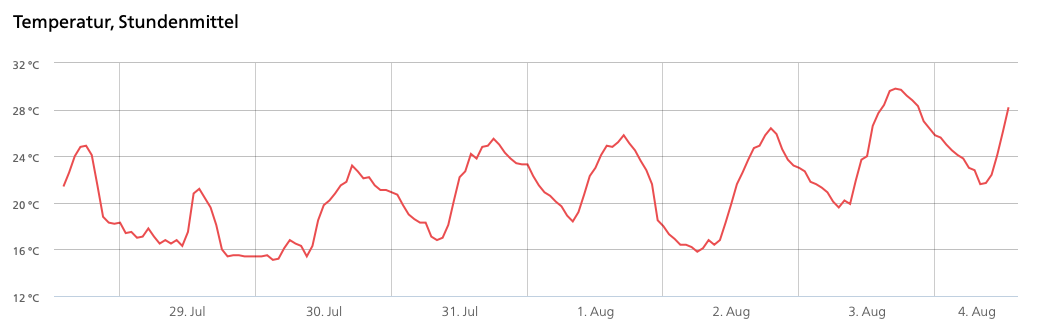
\includegraphics[width=8cm]{temperaturverlauf.png}
\caption{Temperaturverlauf an der Messstation Lägern ($845$ Meter über Meer) von MeteoSchweiz.}
\label{figure-temperaturverlauf}
\end{minipage}
\hfill
\begin{minipage}{0.3\textwidth}
\centering
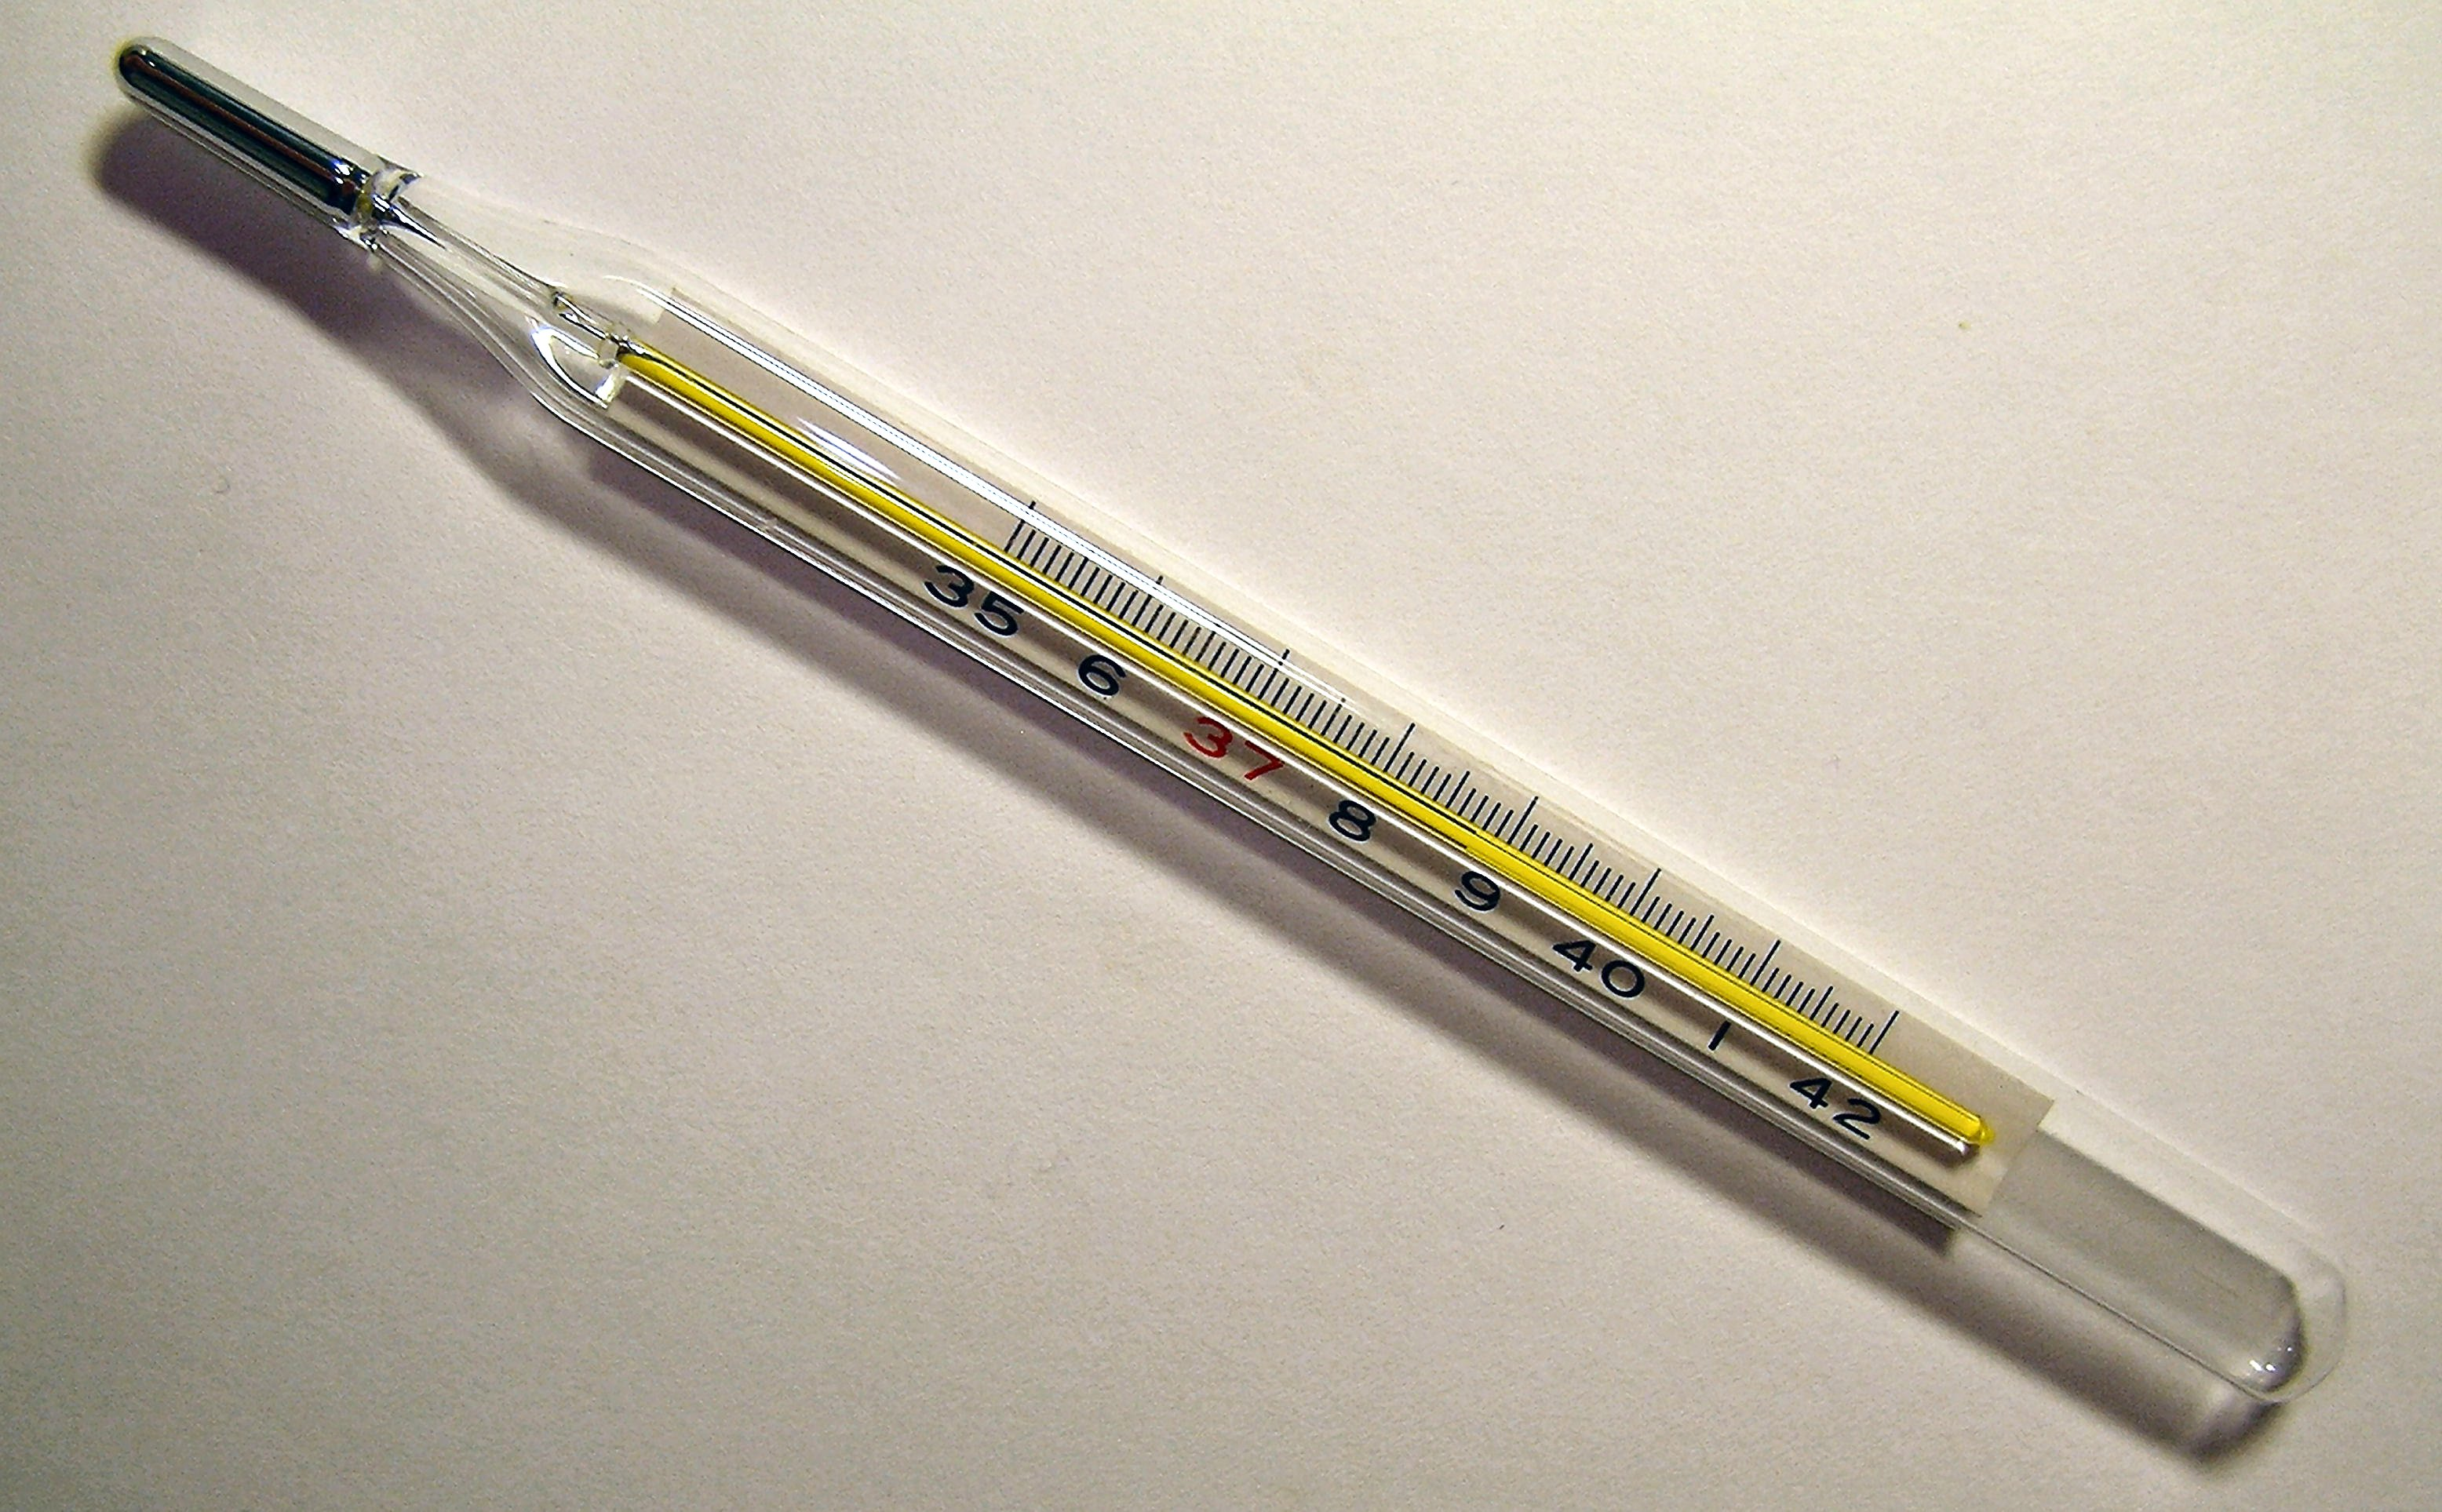
\includegraphics[width=4cm]{qucksilberthermometer.jpg}
\caption{Klassisches Quecksilberthermometer zur Messung der Temperatur.}
\label{figure-quecksilberthermometer}
\end{minipage}
\end{figure}

Beobachten wir etwa die Lufttemperatur an einem Sommertag von $1$ Uhr bis $23$ Uhr. Morgens um $1$ Uhr beträgt die Temperatur $\qty{18}{\degreeCelsius}$. Danach steigt die Temperatur auf $\qty{26}{\degreeCelsius}$ bevor sie nachts wieder auf $\qty{23}{\degreeCelsius}$ sinkt. Dabei steigt die Temperatur nicht sprunghaft an, sondern die Luft durchläuft alle Temperaturen, die zwischen $\qty{18}{\degreeCelsius}$ und $\qty{23}{\degreeCelsius}$ liegen. Es werden also unendlich viele Temperaturen durchlaufen. Dies gilt auch für das Absenken der Temperatur. Die Temperatur ist also eine analoge Grösse. Ein Quecksilberthermometer (siehe \autoref{figure-quecksilberthermometer}) ist ein analoges Messgerät, da die Flüssigkeit (zumindest theoretisch) jede beliebige Temperatur anzeigen kann (auch wenn wir nicht jeden Wert exakt ablesen können).

\end{example}

\begin{example}
~
\begin{figure}[htb]
\begin{minipage}[t]{0.65\textwidth}
\vspace{0pt} 
Beschleunigt ein Auto von  \qty[per-mode = fraction]{0}{\km\per\hour} auf  \qty[per-mode = fraction]{100}{\km\per\hour}, dann durchläuft das Auto alle Geschwindigkeiten zwischen diesen beiden Werten. Es wird kein Wert übersprungen, die Geschwindigkeit kann zu jedem Zeitpunkt gemessen werden. Die Geschwindigkeit ist somit eine analoge Grösse. Ein Tachometer mit einem Zeiger (siehe \autoref{figure-tacho}), so wie es typischerweise in Autos verbaut ist, ist ein analoges Messgerät. Wir können die Geschwindigkeit prinzipiell beliebig genau ablesen.
\end{minipage}
\hfill
\begin{minipage}[t]{0.3\textwidth}
\vspace{0pt} 
\centering
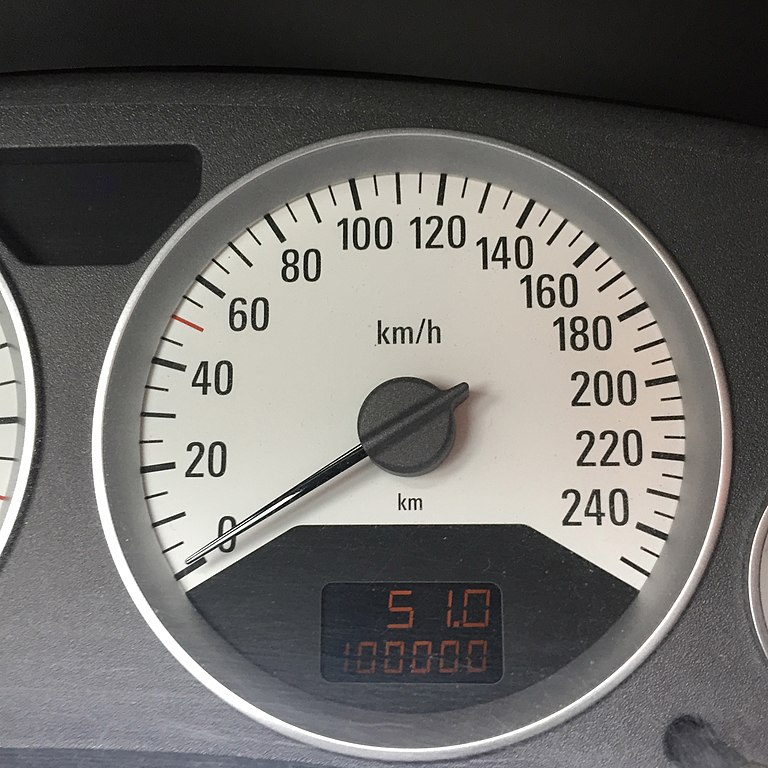
\includegraphics[height=2cm]{tacho.jpg}
\caption{Tachometer mit analoger Geschwindigkeitsanzeige und digitalem Kilometerzähler.}
\label{figure-tacho}
\end{minipage}
\end{figure}

\end{example}

\section{Digitale Daten}

Bei digitalen Daten können nur ganz bestimmte, isolierte Werte vorkommen.

\begin{definition}[Digitale Daten]
Werden Daten nur durch eine Folge von Zeichen dargestellt, dann handelt es sich um digitale Daten.
\end{definition}

Diese Definition ist sehr allgemein. Daraus ergibt sich, dass digitale Daten auch \textbf{ohne} ein elektronisches Gerät existieren.

\begin{example}
Der (vereinfachte) Aufbau der \ac{DNA} wird durch eine Kombination der vier Basen Adenin (A), Thymin (T), Cytosin (C) und Guanin (G) beschrieben. Es ist somit eine Folge der Zeichen A, T, C und G. Notiert man den Aufbau durch diese Zeichen, dann handelt es sich um digitale Daten.
\end{example}

\begin{example}
Das Morsealphabet besteht aus kurzen und langen Tönen sowie verschieden langen Pausen. Die Töne werden durch Striche und Punkte dargestellt. Buchstaben werden durch eine Folge von Strichen und Punkten konstruiert. Es handelt sich somit um digitale Daten.
\end{example}

Natürlich sind alle Daten, die ein Computer verarbeitet auch digitale Daten. Die Besonderheit bei den Daten die ein Computer verarbeitet besteht darin, dass ausschliesslich die Ziffern $0$ und $1$ zum Einsatz kommen.

\section{Binärdaten}

Computer verarbeiten digitale Daten mit zwei klar unterscheidbaren Zeichen. Die gebräuchlichste Darstellung für die zwei Zeichen sind die Ziffern $0$ und $1$.

\begin{definition}[Binärdaten]
Digitale Daten die nur aus den Ziffern $0$ und $1$ bestehen nennen wir Binärdaten. Computer verarbeiten Binärdaten.
\end{definition}

\begin{definition}[Binärziffer]
Die Ziffern $0$ und $1$ werden Binärziffern (eng. binary digit) oder kurz \textbf{Bit} genannt. Ein Bit kann also zwei verschiedene Werte annehmen. Eine Folge von Bits bezeichnen wir somit als Binärdaten.
\end{definition}

\begin{example}
Die Binärdaten \texttt{00110010001100000011000000110001001110100010000001} \\ \texttt{00000100100000010100110111000001100001011000110110010100100000010011110110} \\ \texttt{01000111100101110011011100110110010101111001} bestehen aus $168$ Bits.
\end{example}